\chapter{مشتقات الأحماض الكربوكسيلية}\label{ch:b2:acyl-substitution}

اغلِ زيت الزيتون مع هيدروكسيد الصوديوم تحصل على الصابون والغليسرول: وهذا
أقدم تفاعل عضوي أُجري عن قصد. فالزيت إستر للغليسرول 
وأحماض طويلة السلسلة، والهيدروكسيد يقطع كل إستر عند رابطة واحدة، هي دائمًا
الرابطة نفسها، بين كربون الكربونيل وأكسجين الكحول. والإسترات،
والأحماض، والأميدات، والأنهيدريدات، وكلوريدات الأسيل كلها تتفاعل على هذا النحو:
يُضاف محب للنواة إلى كربون الكربونيل، وتغادر مجموعة. وترتيب هذه
المركبات بحسب سهولة مغادرة مجموعتها يبيّن أيها يمكن تحويله إلى أيها،
وفي أي اتجاه يجب على الكيميائي أن يصعد.

\begin{recall}
مجلد السنة الأولى: التنشيط المحب للإلكترونات لمجموعة الكربونيل، وآليتا تكوين نصف الأسيتال
والأسيتال، والإضافات العضوية المغنيزيومية، ومانحات الهيدريد ومجال استعمالها، والمجموعات المغادرة،
و$\mathrm pK_a$، و$Q$ و$K$. و\cref{ch:b2:amines}: \omterm{def:b2:amines:nucleophilic-addition}{الإضافة المحبة للنواة}، والأمينات.
و\cref{ch:b2:equilibrium-shifts}: إزاحة التوازن. والمجلد المدرسي: الإسترات، والأحماض الكربوكسيلية
والأميدات.
\end{recall}

\begin{omfigure}
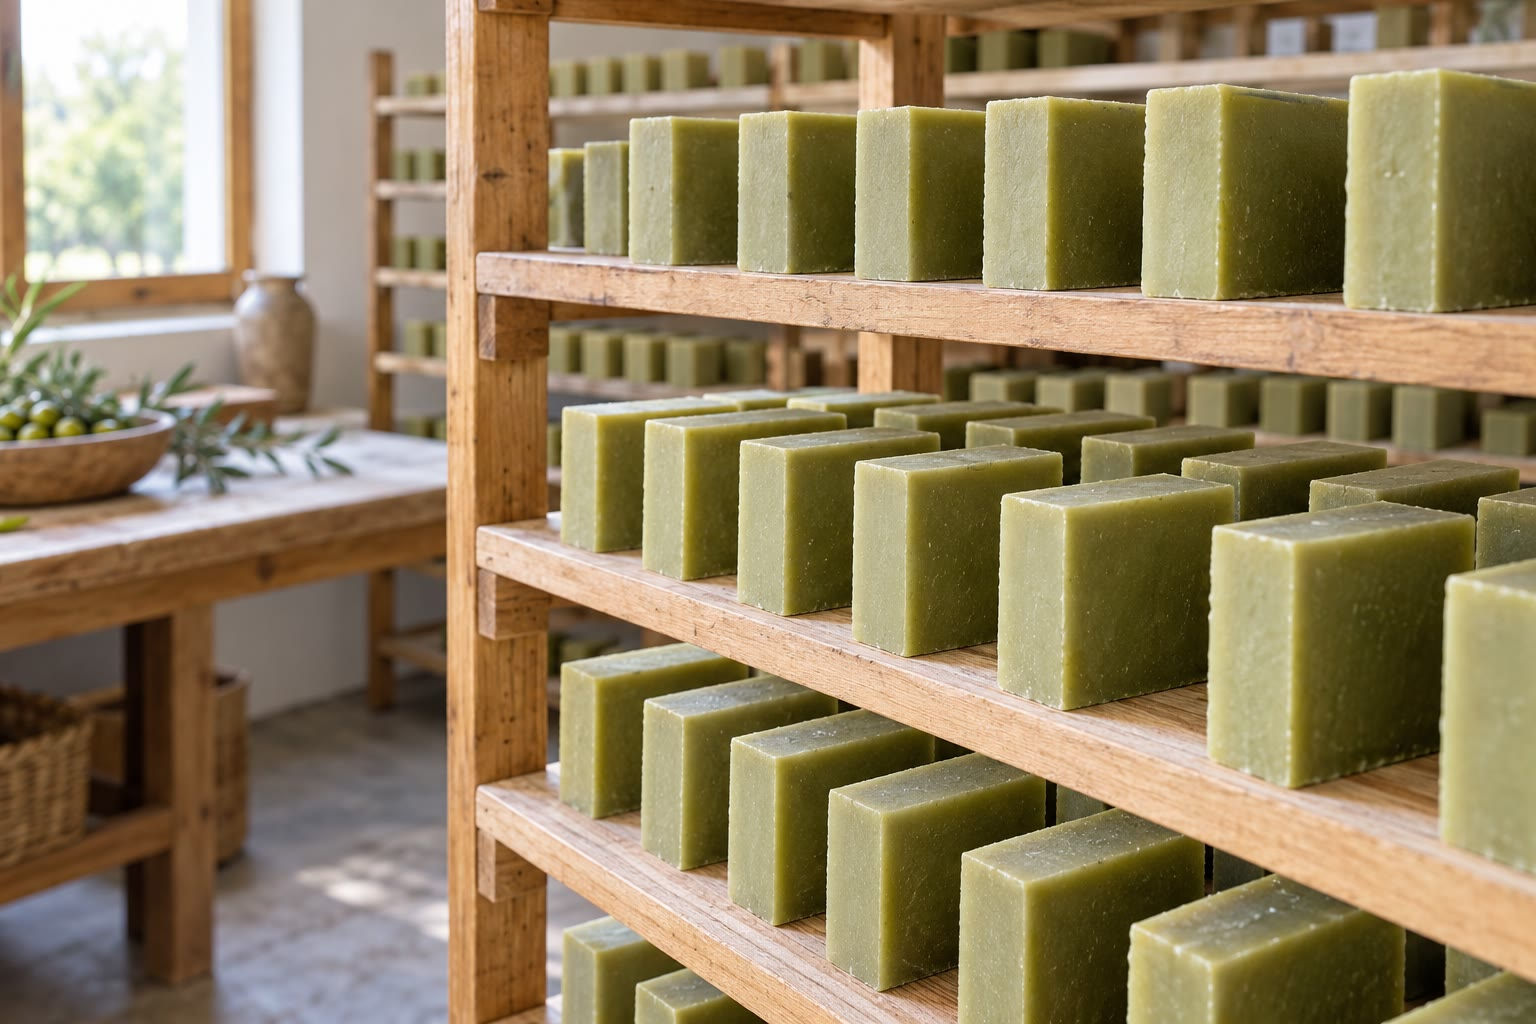
\includegraphics[width=0.58\linewidth]{images/book3/ai/b2-24-soap-bars.jpg}

{\small قطع من صابون زيت الزيتون تجف على رفوف خشبية. والصابون ملح الصوديوم للأحماض الدهنية
المتحررة حين يُغلى الزيت، وهو إستر، مع هيدروكسيد الصوديوم.}
\end{omfigure}

\section{العائلة وتفاعليتها}

\begin{definition}[مشتقات الأحماض الكربوكسيلية]\label{def:b2:acyl-substitution:derivative}
\emph{مشتق الحمض الكربوكسيلي}\index{مشتق حمض كربوكسيلي} مركب \ce{R-CO-Z}
استُبدلت فيه بمجموعة \ce{OH} لحمض كربوكسيلي مجموعة أخرى Z. و\emph{مجموعة
الأسيل}\index{مجموعة أسيل} $\mathrm{R{-}CO{-}}$ مشتركة بينها كلها. ففي \emph{كلوريد الأسيل}\index{كلوريد أسيل}،
Z هي Cl؛ وفي \emph{أنهيدريد الحمض}\index{أنهيدريد حمض}، Z هي $\mathrm{O{-}CO{-}R'}$، أي مجموعتا أسيل
تتقاسمان أكسجينًا واحدًا؛ وفي الإستر Z هي $\mathrm{OR'}$، وفي الأميد $\mathrm{NR'_2}$.
\end{definition}

\begin{proposition}[سلّم التفاعلية]\label{prop:b2:acyl-substitution:reactivity}
تجاه المحبات للنواة، تتفاعل المشتقات بالترتيب \babelsublr{\foreignlanguage{arabic}{\omterm{def:b2:acyl-substitution:derivative}{كلوريد الأسيل}}~$>$~\foreignlanguage{arabic}{الأنهيدريد}~$>$~\foreignlanguage{arabic}{الإستر}
$\approx$~\foreignlanguage{arabic}{الحمض}~$>$~\foreignlanguage{arabic}{الأميد}}.
\end{proposition}

\begin{proof}[تعليل]
يتضافر أثران. فالمجموعة المغادرة \ce{Z-} تغادر بسهولة أكبر كلما كانت قاعدة أضعف:
\ce{Cl-} (حمضه المرافق \ce{HCl}، و$\mathrm pK_a$ نحو $-7$) أفضل بكثير من الكربوكسيلات
($\mathrm pK_a$ نحو 5)، أو الألكوكسيد (نحو 16) أو أيون الأميد (نحو 35). ثم إن المجموعة Z تمنح
الكربونيل كثافة إلكترونية بالمنح الميزوميري لزوجها الحر، مما يجعل كربون الكربونيل
أقل محبة للإلكترونات: وهو منح ضعيف للكلور، وأقوى ما يكون للنيتروجين. فالأميد هو في آن واحد أضعف
المحبات للإلكترونات وأردأ المجموعات المغادرة.
% ledger: pka:ethanoic, pka:ethanol
\end{proof}

\section{الاستبدال الأسيلي المحب للنواة}

\begin{definition}[الاستبدال الأسيلي المحب للنواة]\label{def:b2:acyl-substitution:nas}
\emph{الاستبدال الأسيلي المحب للنواة}\index{استبدال أسيلي محب للنواة} يستبدل بالمجموعة Z
في مركب أسيلي محبًا للنواة. ويجري بإضافة المحب للنواة إلى كربون الكربونيل،
معطيًا \emph{وسيطًا رباعي الأوجه}\index{وسيط رباعي الأوجه}، يتبعها
حذف المجموعة المغادرة، الذي يعيد الرابطة \ce{C=O}.
\end{definition}

\begin{proposition}[الإضافة--الحذف]\label{prop:b2:acyl-substitution:addition-elimination}
يمر الاستبدال الأسيلي \omterm{def:b2:acyl-substitution:nas}{بوسيط رباعي الأوجه}؛ ويُسرَّع في القاعدة بمحب للنواة أقوى
وفي الحمض بتنشيط الكربونيل.
\end{proposition}

\begin{proof}[تعليل]
كربون الكربونيل، المستوي والمحب للإلكترونات، يستقبل المحب للنواة من فوق مستويه أو من
تحته، كما في إضافات \cref{ch:b2:amines}؛ ومع مجموعة Z قادرة على المغادرة، يطرد الوسيط
هذه المجموعة بدلًا من أن يُبرتَن. وفي القاعدة يكون المحب للنواة أنيونًا (\ce{HO-}،
\ce{RO-})؛ وفي الحمض يُبرتن أكسجين الكربونيل ويكفي محب للنواة متعادل (الماء، الكحول).
والإسترات الموسومة بالنظير \ce{^{18}O} في جزئها الكحولي تعطي، بالحلمهة، كحولًا موسومًا
وحمضًا غير موسوم: فالرابطة المنكسرة هي رابطة الأسيل--الأكسجين، كما تقتضي الآلية.
\end{proof}

\begin{omfigure}
\setchemfig{atom sep=1.7em}
\schemestart
\chemfig{R-C(=[2]O)-OR'} \+ \chemfig{HO^{-}}
\arrow{->[إضافة]}
\chemfig{R-C(-[2]O^{-})(-[6]OH)-OR'}
\arrow{->[حذف]}[,1.3]
\chemfig{R-C(=[2]O)-OH} \+ \chemfig{^{-}OR'}
\schemestop

\medskip
\schemestart
\chemfig{R-C(=[2]O)-OH} \+ \chemfig{^{-}OR'}
\arrow{->[انتقال بروتون]}
\chemfig{R-C(=[2]O)-O^{-}} \+ \chemfig{HOR'}
\schemestop
\par\vspace{6pt}

{\small \omterm{def:b2:acyl-substitution:saponification}{تصبّن} إستر. يُضاف الهيدروكسيد إلى كربون الكربونيل، معطيًا \omterm{def:b2:acyl-substitution:nas}{الوسيط الرباعي
الأوجه}؛ ثم يغادر الألكوكسيد وتتكوّن الرابطة \ce{C=O} من جديد؛ ثم يأخذ الألكوكسيد، وهو قاعدة قوية،
بروتون الحمض. وهذه الخطوة الأخيرة تجعل التفاعل تامًا.}
\end{omfigure}

\begin{method}[رسم استبدال أسيلي]\label{met:b2:acyl-substitution:nas-mechanism}
\begin{enumerate}
  \item في القاعدة: يُضاف المحب للنواة الأنيوني إلى كربون الكربونيل؛ وتذهب الشحنة السالبة إلى
        الأكسجين؛ ثم تتكوّن الرابطة \ce{C=O} من جديد وتغادر Z؛ واختم بأي خطوة حمض--قاعدة.
  \item في الحمض: برتِن أكسجين الكربونيل؛ ثم يُضاف المحب للنواة المتعادل؛ وانقل بروتونًا
        إلى المجموعة المغادرة؛ فتغادر جزيئًا متعادلًا؛ ثم انزع البروتون من الكربونيل.
  \item عُدّ الخطوات: كل وسيط إما رباعي الأوجه وإما مركب كربونيلي.
\end{enumerate}
\end{method}

\section{الإسترات}

\begin{definition}[الأسترة]\label{def:b2:acyl-substitution:esterification}
\emph{الأسترة}\index{أسترة} تكوّن إسترًا من حمض كربوكسيلي (أو من مشتق أكثر
تفاعلية) وكحول. والتفاعل المباشر لحمض مع كحول، المحفَّز بحمض
قوي، هو أسترة فيشر.
\end{definition}

\begin{proposition}[أسترة فيشر]\label{prop:b2:acyl-substitution:fischer}
\omterm{def:b2:acyl-substitution:esterification}{أسترة} فيشر توازن بطيء، ثابته قرب 4 للكحولات الأولية؛ 
ويُدفع إلى الأمام بفائض من أحد الكاشفين أو بإزالة الماء حال تكوّنه.
\end{proposition}

\begin{proof}[تعليل]
يتوقف الإيثانول وحمض الإيثانويك المتساويان في الكمية حين يتأستر ثلثا الحمض: $K =
(2/3)^2/(1/3)^2 = 4$. ومع الحفاظ على $Q < K$ بفائض من الكحول، أو بتقطير الماء
(جهاز دين--ستارك في مجلد السنة الأولى)، يتقدم التفاعل أكثر
(\cref{ch:b2:equilibrium-shifts}). والخطوات الست للآلية هي خطوات \cref{met:b2:acyl-substitution:nas-mechanism}
في الحمض، وكلها عكوسة.
% ledger: ester:berthelot
\end{proof}

\begin{definition}[التصبّن]\label{def:b2:acyl-substitution:saponification}
\emph{التصبّن}\index{تصبن} هو حلمهة إستر بهيدروكسيد، معطية
ملح الكربوكسيلات والكحول.
\end{definition}

\begin{proposition}[التصبّن تام]\label{prop:b2:acyl-substitution:saponification}
يجري \omterm{def:b2:acyl-substitution:saponification}{التصبّن} حتى نهايته: فخطوته الأخيرة، انتقال البروتون من الحمض الكربوكسيلي إلى
الألكوكسيد، لها ثابت توازن من رتبة $10^{11}$.
\end{proposition}

\begin{proof}
من أجل $\mathrm{RCOOH + R'O^- \to RCOO^- + R'OH}$،
\[
  K = \frac{K_a(\ce{RCOOH})}{K_a(\mathrm{R'OH})} = 10^{\mathrm pK_a(\mathrm{R'OH}) - \mathrm pK_a(\ce{RCOOH})} ;
\]
مع حمض الإيثانويك (4.76) والإيثانول (15.93)، $K = 10^{11.2}$. والكربوكسيلات، وهو محب للإلكترونات ضعيف، لا يهاجمه الكحول: فالتفاعل
الإجمالي لا يعود إلى الوراء.
% ledger: pka:ethanoic, pka:ethanol
\end{proof}

\begin{omfigure}
\setchemfig{atom sep=1.7em}
\schemestart
\chemfig{CH_2(-[0]O-CO-R)-[6]CH(-[0]O-CO-R)-[6]CH_2-[0]O-CO-R}
\+ \chemfig{3\,NaOH}
\arrow{->[تسخين]}
\chemfig{CH_2(-[0]OH)-[6]CH(-[0]OH)-[6]CH_2-[0]OH}
\+ \chemfig{3\,R-COO^{-}\,Na^{+}}
\schemestop
\par\vspace{6pt}

{\small \omterm{def:b2:acyl-substitution:saponification}{تصبّن} ثلاثي غليسريد: تنقطع روابط الإستر الثلاث، فتعطي الغليسرول 
وثلاثة جزيئات من كربوكسيلات الصوديوم، أي الصابون (R سلسلة طويلة، \ce{C17H33} لأوليات
زيت الزيتون).}
\end{omfigure}

\begin{definition}[تبادل الأسترة]\label{def:b2:acyl-substitution:transesterification}
\emph{تبادل الأسترة}\index{تبادل الأسترة} يبادل الجزء الكحولي في إستر،
$\mathrm{RCOOR' + R''OH \rightleftharpoons RCOOR'' + R'OH}$، بحفز حمضي أو قاعدي.
\end{definition}

\begin{definition}[اللاكتونات واللاكتامات]\label{def:b2:acyl-substitution:lactone}
\emph{اللاكتون}\index{لاكتون} إستر حلقي، يتكوّن \omterm{def:b2:acyl-substitution:esterification}{بأسترة} داخلية لحمض
هيدروكسيلي؛ و\emph{اللاكتام}\index{لاكتام} أميد حلقي.
\end{definition}

\section{المشتقات المنشطة}

النزول على سلّم التفاعلية سهل: \omterm{def:b2:acyl-substitution:derivative}{فكلوريد الأسيل} يعطي أنهيدريدًا أو إسترًا أو
أميدًا مع المحب للنواة المناسب، وغالبًا في درجة حرارة الغرفة. أما الصعود فيحتاج إلى تنشيط: إذ
يحوَّل الحمض الكربوكسيلي إلى كلوريده بكلوريد الثيونيل،
\[
  \ce{RCOOH + SOCl2 -> RCOCl + SO2 + HCl} ,
\]
ونواتجه الثانوية غازات. ثم يتفاعل \omterm{def:b2:acyl-substitution:derivative}{كلوريد الأسيل} مع كحول أو أمين؛ وتحتجز قاعدةٌ
(البيريدين، أو ثلاثي إيثيل أمين، أو مكافئ ثانٍ من الأمين) \ce{HCl} المتكوّن، الذي
كان سيبرتن الأمين لولا ذلك.

\begin{method}[التنقل بين المشتقات]\label{met:b2:acyl-substitution:ladder}
\begin{enumerate}
  \item نزولًا على السلّم (\babelsublr{\foreignlanguage{arabic}{كلوريد}~$\to$~\foreignlanguage{arabic}{أنهيدريد}~$\to$~\foreignlanguage{arabic}{إستر}، \foreignlanguage{arabic}{حمض}~$\to$~\foreignlanguage{arabic}{أميد}}): عالِج بالمحب
        للنواة، مع قاعدة لاحتجاز الحمض المتحرر.
  \item صعودًا على السلّم: حوّل الحمض أولًا إلى الكلوريد (\ce{SOCl2})؛ أما الإستر أو الأميد فيُحلمه
        أولًا إلى الحمض.
  \item بين حمض وإستر: \omterm{def:b2:acyl-substitution:esterification}{أسترة} فيشر (توازن) أو \omterm{def:b2:acyl-substitution:saponification}{تصبّن}
        (تام) يتبعه تحميض.
\end{enumerate}
\end{method}

\begin{omfigure}
\begin{tikzpicture}[font=\small, >={Stealth}]
  \foreach \y/\n in {4/{\foreignlanguage{arabic}{كلوريد الأسيل \ce{RCOCl}}}, 3/{\foreignlanguage{arabic}{أنهيدريد \ce{(RCO)2O}}}, 2/{\foreignlanguage{arabic}{إستر $\mathrm{RCOOR'}$ \quad حمض \ce{RCOOH}}}, 1/{\foreignlanguage{arabic}{أميد $\mathrm{RCONR'_2}$}}} {
    \node[cyclenode, minimum width=5.2cm] at (0,\y*1.1) {\n};
  }
  \draw[->, thick, omDef] (-3.1,4.3) -- (-3.1,1.1) node[midway, left, align=right, font=\scriptsize] {\foreignlanguage{arabic}{سهل:}\\ \foreignlanguage{arabic}{محب للنواة}\\ \foreignlanguage{arabic}{+ قاعدة}};
  \draw[->, thick, omThm] (3.1,2.2) -- (3.1,4.4) node[midway, right, align=left, font=\scriptsize] {\foreignlanguage{arabic}{صعود:}\\ \foreignlanguage{arabic}{عبر الحمض}\\ \foreignlanguage{arabic}{و\ce{SOCl2}}};
  \node[font=\scriptsize, anchor=south] at (0,4.85) {\foreignlanguage{arabic}{أكثر تفاعلية}};
  \node[font=\scriptsize, anchor=north] at (0,0.55) {\foreignlanguage{arabic}{أقل تفاعلية}};
\end{tikzpicture}

{\small سلّم تفاعلية مشتقات الأحماض الكربوكسيلية. يمكن تحويل أي مشتق إلى
مشتق أدنى منه بمحب للنواة؛ أما الصعود فيمر عبر الحمض وكلوريده.}
\end{omfigure}

\section{المركبات العضوية الفلزية والهيدريدات}

\begin{proposition}[إضافتا غرينيار]\label{prop:b2:acyl-substitution:grignard-ester}
الإستر المعالج بفائض من كاشف عضوي مغنيزيومي يعطي كحولًا ثالثيًا يحمل مجموعتين
متماثلتين مصدرهما الكاشف.
\end{proposition}

\begin{proof}[تعليل]
تعطي الإضافة الأولى \omterm{def:b2:acyl-substitution:nas}{وسيطًا رباعي الأوجه} يطرد الألكوكسيد: فينتج كيتون. والكيتون
أكثر محبة للإلكترونات من الإستر (لا منح ميزوميري من مجموعة $\mathrm{OR'}$) فيتفاعل مع
الكاشف أسرع من الإستر المتبقي؛ والإضافة الثانية، إلى الكيتون، تعطي ألكوكسيد
كحول ثالثي، تبرتنه المعالجة الحمضية. ولا يمكن إيقاف التفاعل عند الكيتون.
\end{proof}

\begin{proposition}[الاختزالات بالهيدريدات]\label{prop:b2:acyl-substitution:hydrides}
يختزل هيدريد الليثيوم والألومنيوم الإسترات والأحماض إلى كحولات أولية، والأميدات إلى أمينات؛
أما بوروهيدريد الصوديوم فيختزل الألدهيدات والكيتونات لا الإسترات ولا الأحماض ولا الأميدات. وهيدريد
ألومنيوم ضخم (DIBAL-H) عند \qty{-78}{\degreeCelsius} يختزل الإستر إلى الألدهيد.
\end{proposition}

\begin{proof}[تعليل]
\ce{LiAlH4} مانح هيدريد قوي: فهو مثل كاشف غرينيار يُضاف مرتين إلى الإستر (عبر
الألدهيد). أما البوروهيدريد فأضعف من أن يختزل كربونيل الإستر الأقل محبة للإلكترونات. ومع DIBAL-H في
درجة حرارة منخفضة لا يطرد \omterm{def:b2:acyl-substitution:nas}{الوسيط الرباعي الأوجه}، الممسوك بالألومنيوم، الألكوكسيدَ حتى
المعالجة المائية، حين لا يبقى هيدريد: فيبقى الألدهيد. وفي الأميد، يُحذف الأكسجين،
المرتبط بالألومنيوم، بدلًا من النيتروجين، فيبقى أيون إيمينيوم يختزله
الهيدريد إلى الأمين.
\end{proof}

\begin{history}[شوفرول والدهون]
\begin{minipage}[t]{0.22\linewidth}
\vspace{0pt}
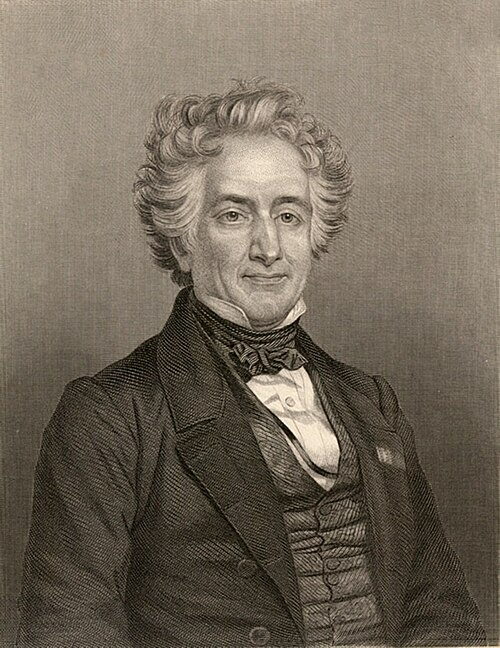
\includegraphics[width=\linewidth]{images/book3/chevreul.jpg}
\end{minipage}\hfill
\begin{minipage}[t]{0.74\linewidth}
\vspace{0pt}
بيّن ميشيل أوجين شوفرول، في دراسة نُشرت سنة 1823، أن الدهون مركبات من الغليسرول
مع أحماض دهنية، عزلها وسمّاها (أحماض الستياريك والأولييك والبوتيريك)، وأن
\omterm{def:b2:acyl-substitution:saponification}{التصبّن} يقسمها إلى هذين الجزأين. وقد حوّل عمله صناعة الصابون والشموع إلى
كيمياء؛ وعاش حتى بلغ 102 من العمر. (صورة شخصية بريشة نيكولا أوستاش موران، ملكية عامة، ويكيميديا
كومنز.)
\end{minipage}
\end{history}

\begin{safety}{\ghs[5mm]{GHS02}\,\ghs[5mm]{GHS05}\,\ghs[5mm]{GHS06}}
يتفاعل كلوريد الثيونيل وكلوريدات الأسيل بعنف مع الماء ويطلقان غازات أكّالة؛ فتُتداول
جافة، تحت ساحبة أبخرة. وهيدريد الليثيوم والألومنيوم يشتعل عند ملامسة الماء؛ ويُتلف
فائضه بحذر في النهاية. وهيدروكسيد الصوديوم المركز أكّال للجلد 
والعينين. والميثانول سام وقابل للاشتعال.
% ledger: ghs:SOCl2, ghs:ethanoyl-chloride, ghs:LiAlH4, ghs:NaOH, ghs:methanol
\end{safety}

\section{تمارين}

\begin{exercise}[$\star$]\label{exo:b2:acyl-substitution:1}
رتّب بحسب التفاعلية تجاه الماء: إيثانوات الإيثيل، وكلوريد الإيثانويل، والإيثانأميد، وأنهيدريد
الإيثانويك.
\end{exercise}

\begin{exercise}[$\star$]\label{exo:b2:acyl-substitution:2}
أعطِ نواتج كلوريد الإيثانويل مع: الماء؛ الإيثانول؛ الأمونيا (مكافئان)؛
إيثانوات الصوديوم؛ ثنائي ميثيل أمين مع ثلاثي إيثيل أمين.
\end{exercise}

\begin{exercise}[$\star$]\label{exo:b2:acyl-substitution:3}
اكتب \omterm{def:b2:acyl-substitution:saponification}{تصبّن} بنزوات الميثيل بهيدروكسيد الصوديوم واحسب كتلة هيدروكسيد
الصوديوم اللازمة لكتلة \qty{13.6}{g} من الإستر.
\end{exercise}

\begin{exercise}[$\star$]\label{exo:b2:acyl-substitution:4}
ارسم \omterm{def:b2:acyl-substitution:lactone}{اللاكتون} الذي يكوّنه حمض 4-هيدروكسي بيوتانويك وأعطِ حجم حلقته.
\end{exercise}

\begin{exercise}[$\star\star$]\label{exo:b2:acyl-substitution:5}
اكتب آلية تفاعل إيثانوات الإيثيل مع الأمونيا.
\end{exercise}

\begin{exercise}[$\star\star$]\label{exo:b2:acyl-substitution:6}
يُصنع الأسبرين من حمض الساليسيليك (حمض 2-هيدروكسي بنزويك) وأنهيدريد الإيثانويك. أي مجموعة
في حمض الساليسيليك تتفاعل، وما الناتج الثانوي؟
\end{exercise}

\begin{exercise}[$\star\star$]\label{exo:b2:acyl-substitution:7}
تُعالج إيثانوات الإيثيل بفائض من بروميد ميثيل المغنيزيوم، ثم بحمض مخفف. أعطِ
الناتج وفسّر لماذا لا يمكن عزل الكيتون.
\end{exercise}

\begin{exercise}[$\star\star$]\label{exo:b2:acyl-substitution:8}
أعطِ ناتج اختزال \omterm{def:b2:acyl-substitution:lactone}{لاكتون} التمرين 4 بواسطة \ce{LiAlH4}.
\end{exercise}

\begin{exercise}[$\star\star$]\label{exo:b2:acyl-substitution:9}
مع $K = 4$، احسب كسر حمض الإيثانويك المتأستر مع مكافئ واحد، ثم مع ثلاثة
مكافئات من الإيثانول. وما الطريقة الأخرى التي تدفع التفاعل؟
\end{exercise}

\begin{exercise}[$\star\star\star$]\label{exo:b2:acyl-substitution:10}
حضّر \textit{N}،\textit{N}-ثنائي إيثيل بنزأميد من حمض البنزويك، وفسّر لماذا يعطي خلط الحمض
مع ثنائي إيثيل أمين والتسخين المعتدل ملحًا بدلًا من ذلك.
\end{exercise}

\begin{exercise}[$\star\star\star$]\label{exo:b2:acyl-substitution:11}
قرينة \omterm{def:b2:acyl-substitution:saponification}{التصبّن} لدهن هي كتلة هيدروكسيد البوتاسيوم، بوحدة mg، اللازمة \omterm{def:b2:acyl-substitution:saponification}{لتصبين}
\qty{1}{g} منه. احسبها للتريولين (\qty{885.4}{g/mol}؛ KOH \qty{56.11}{g/mol}).
\end{exercise}

\begin{exercise}[$\star\star\star$]\label{exo:b2:acyl-substitution:12}
جزيء يحمل إسترًا وأميدًا وكيتونًا. أي مجموعة (أو مجموعات) يختزلها \ce{NaBH4}، وأيها يختزلها
\ce{LiAlH4}؟ وماذا تحصل في كل حالة؟
\end{exercise}

\section{مسألة: وقود الديزل الحيوي من زيت القلي}

\begin{problem}[{مسألة نهاية الأسبوع --- التريولين وكتلته المولية، وتبادل الأسترة مع
الميثانول ودور القاعدة، والتفاعل الجانبي مع الأحماض الحرة والماء، والمردودات لكل
طن من الزيت}]
\label{pb:b2:acyl-substitution:1}
اعتبر الزيت تريولينًا نقيًا، وهو ثلاثي غليسريد حمض الأولييك (\ce{C17H33COOH}). والكتل المولية
(\unit{g/mol}): C 12.011، H 1.008، O 15.999، Na 22.990. والغليسرول هو بروبان-1،2،3-تريول.
% ledger: aw:C, aw:H, aw:O, aw:Na, ghs:methanol, ghs:NaOH

\medskip
\noindent\textbf{الجزء الأول --- التريولين.}
\begin{enumerate}
  \item أعطِ صيغة حمض الأولييك وصيغة الغليسرول.
  \item اكتب صيغة التريولين واحسب كتلته المولية.
  \item كم مجموعة إستر يحوي؟
  \item لحمض الأولييك رابطة مزدوجة cis واحدة. لماذا تكون الزيوت الغنية به سائلة في درجة حرارة الغرفة؟
  \item ماذا يعطي \omterm{def:b2:acyl-substitution:saponification}{تصبّن} التريولين؟
  \item ما الديزل الحيوي من الناحية الكيميائية؟
\end{enumerate}

\medskip
\noindent\textbf{الجزء الثاني --- \omterm{def:b2:acyl-substitution:transesterification}{تبادل الأسترة}.}
\begin{enumerate}[resume]
  \item اكتب \omterm{def:b2:acyl-substitution:transesterification}{تبادل الأسترة} بين التريولين والميثانول.
  \item لماذا تُستعمل قاعدة (ميثوكسيد الصوديوم أو هيدروكسيده) حفازًا؟
  \item ارسم \omterm{def:b2:acyl-substitution:nas}{الوسيط الرباعي الأوجه} للتبادل الأول.
  \item لماذا يُستعمل الميثانول بفائض (ستة مكافئات بدل ثلاثة)؟
  \item الغليسرول لا يمتزج بإسترات الميثيل. كيف يساعد ذلك؟
  \item هل يُستهلك الحفاز في التفاعل المثالي؟
\end{enumerate}

\medskip
\noindent\textbf{الجزء الثالث --- الأحماض الحرة والماء.}
\begin{enumerate}[resume]
  \item يحوي زيت القلي المستعمل حمض أولييك حرًا. ماذا يفعل بالقاعدة؟
  \item ماذا يفعل الماء بإسترات الميثيل بوجود القاعدة؟
  \item لماذا يكون الصابون المتكوّن مزعجًا؟
  \item كيف يمكن إزالة الأحماض الحرة أولًا، دون قاعدة؟
  \item لماذا يجب تجفيف الزيت قبل التفاعل؟
\end{enumerate}

\medskip
\noindent\textbf{الجزء الرابع --- لكل طن من الزيت.}
\begin{enumerate}[resume]
  \item احسب كمية التريولين في طن واحد.
  \item احسب كتلة الميثانول المستهلكة.
  \item احسب كتلة أوليات الميثيل المتكوّنة.
  \item تحقق من انحفاظ الكتلة.
  \item يُعالج زيت فيه 2~\% كتلةً من حمض الأولييك الحر بهيدروكسيد الصوديوم: احسب كتلة
        هيدروكسيد الصوديوم التي يستهلكها الحمض لكل طن.
  \item احسب كتلة الغليسرول المنتَج معه لكل طن من التريولين.
\end{enumerate}
\end{problem}
